% Neighborhood-order figure for the TorchSOM documentation.
% Mirrors the JMLR paper (Appendix B): rectangular Chebyshev blocks (left) and
% hexagonal hop-distance rings (right) around the BMU, for orders o = 1, 2, 3.
%
% Regenerate the PNG with:
%   pdflatex topologies.tex
%   pdftocairo -png -singlefile -r 300 topologies.pdf ../source/_static/som/topologies
\documentclass[tikz,border=6pt]{standalone}
\usepackage{amssymb}
\usetikzlibrary{shapes.geometric}

% Colour-coding for the BMU and neighborhood orders (matches the paper).
\colorlet{bmucolor}{black!80}
\colorlet{order1color}{blue!60}
\colorlet{order2color}{teal!60}
\colorlet{order3color}{purple!40}

% Fill a unit grid cell with a 1% margin.
\newcommand{\fillrect}[3]{%
    \fill[#3] (#1+0.01,#2+0.01) rectangle ++ (0.98,0.98);
}

\begin{document}
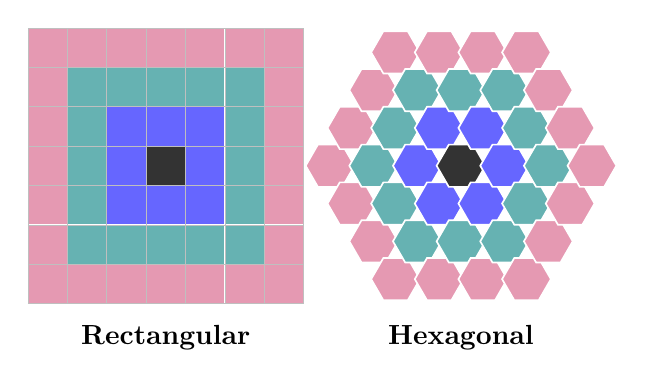
\begin{tikzpicture}
    % --- Rectangular grid (left): Chebyshev (max-norm) blocks ---
    \begin{scope}[scale=0.5]
        \foreach \x in {1,...,7} {
                \foreach \y in {1,...,7} {
                        \pgfmathtruncatemacro{\ord}{max(abs(\x-4),abs(\y-4))}
                        \ifcase\ord
                            \fillrect{\x}{\y}{bmucolor}\or
                            \fillrect{\x}{\y}{order1color}\or
                            \fillrect{\x}{\y}{order2color}\or
                            \fillrect{\x}{\y}{order3color}
                        \fi
                    }
            }
        \draw[step=1, gray!50, very thin] (1,1) grid (8,8);
        \node[font=\bfseries, anchor=north] at (4.5,0.7) {Rectangular};
    \end{scope}
    % --- Hexagonal grid (right): hop-distance rings ---
    \begin{scope}[xshift=6cm, yshift=2.25cm]
        \foreach \q in {-3,...,3} {
                \foreach \r in {-3,...,3} {
                        \pgfmathtruncatemacro{\hd}{(abs(\q)+abs(\r)+abs(\q+\r))/2}
                        \ifnum\hd<4
                            \pgfmathsetmacro{\hx}{0.32*sqrt(3)*(\q+\r/2)}
                            \pgfmathsetmacro{\hy}{0.32*1.5*\r}
                            \ifcase\hd
                                \node[regular polygon, regular polygon sides=6, fill=bmucolor, minimum size=0.62cm, inner sep=0pt, draw=white, line width=0.6pt] at (\hx,\hy) {}; \or
                                \node[regular polygon, regular polygon sides=6, fill=order1color, minimum size=0.62cm, inner sep=0pt, draw=white, line width=0.6pt] at (\hx,\hy) {}; \or
                                \node[regular polygon, regular polygon sides=6, fill=order2color, minimum size=0.62cm, inner sep=0pt, draw=white, line width=0.6pt] at (\hx,\hy) {}; \or
                                \node[regular polygon, regular polygon sides=6, fill=order3color, minimum size=0.62cm, inner sep=0pt, draw=white, line width=0.6pt] at (\hx,\hy) {};
                            \fi
                        \fi
                    }
            }
        \node[font=\bfseries, anchor=north] at (0,-1.9) {Hexagonal};
    \end{scope}
\end{tikzpicture}
\end{document}
